
\subsection{Zoeken}\label{zoeken}

Voor \drupalpath wordt de \emph{Solr module} gebruikt, deze module vervangt de standaard \emph{Drupal Search module}. 
De \emph{Solr module} biedt naast de standaard zoek functionaliteit ook meer geavanceerde functionaliteiten zoals zoeken in bijlagen, markeren van zoekwoorden en de mogelijkheid tot het aanpassen van de \emph{Bias settings}. 

\subsubsection{Bias settings}

\emph{Bias settings} maken het mogelijk inhoud voorrang te geven in de zoekresultaten. Je kunt bijvoorbeeld het inhoudstype \emph{Nieuws} meer punten geven dan het inhoudstype \emph{Bekendmaking}. Hoe hoger het aantal toegekende punten hoe meer voorrang het krijgt. 

Ga naar \drupalpath{admin/config/search/apachesolr} en klik vervolgens op \emph{Bias} bij de betreffende website om de \emph{Bias settings} aan te passen. Let op: het is niet aangeraden om zonder voldoende kennis deze settings aan te passen.

\begin{center}
	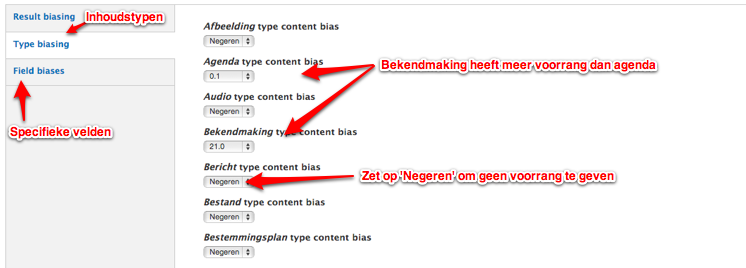
\includegraphics[width=\textwidth]{img/bias.png}
\end{center}

Klik na het bewerken op de knop \emph{Instellingen opslaan} om de \emph{Bias settings} op te slaan. 